\documentclass[t]{beamer}
\usepackage{hyperref}
% Load general definitions
% Preamble file - general definitions, package loading, etc.

%=================================
% Load packages
\usepackage{amssymb,amsmath}
\usepackage{graphicx}
\usepackage{url}
\usepackage{tikz}
\usetikzlibrary{mindmap,trees,arrows}
\usepackage{fancyvrb}
\usepackage[portuguese]{babel} 
\usepackage[utf8]{inputenc}
\usepackage{subfigure}
\usepackage{times}
\usepackage[T1]{fontenc}
\usepackage{cancel}
\usepackage{color}
\usepackage{listings}
\usepackage[document]{ragged2e}

%=================================
% Set mode
\mode<presentation>
{
	\usetheme{Madrid}
	\usecolortheme{structure}
	\useoutertheme{infolines}
	\setbeamercovered{invisible}
}

% Get rid of nav bar
\beamertemplatenavigationsymbolsempty

% Insert frame number at bottom of the page.
\usefoottemplate{\hfil\tiny{\color{black!90}\insertframenumber}} 

%=================================
% Define new commands

\newcommand\Real{{\mathbb{R}}}
%\newcommand{\vi}{\vspace{0.6\baselineskip}}
%\newcommand{\goodgap}{\hspace{\subfigtopskip}\hspace{\subfigbottomskip}}


% Equation environments
\newcommand{\beq}{\begin{equation}}
\newcommand{\eq}{\end{equation}}
\newcommand{\beqs}{\begin{equation*}}
\newcommand{\eqs}{\end{equation*}}
\newcommand{\beqn}{\begin{eqnarray}}
\newcommand{\eqn}{\end{eqnarray}}
% Bold variables
\newcommand{\mbf}[1]{\ensuremath{\mathbf{#1}}}
% Itemization
\newcommand{\bitem}{\begin{itemize}}
\newcommand{\eitem}{\end{itemize}}
\newcommand{\spitem}{\vskip 1em\item}
\newcommand{\bitems}{\begin{itemize}\item}
\newcommand{\benums}{\begin{enumerate}\item}
\newcommand{\eenum}{\end{enumerate}}
% color blocks
\newenvironment{colorblock}[2]{%
\setbeamercolor{block title}{#2}
\begin{block}{#1}}{\end{block}}
% Vertical spacing
\newcommand{\vone}{\vskip 1em}
\newcommand{\vhalf}{\vskip .5em}
% Frame environments
\newenvironment{ftst}[3][t]{%
\begin{frame}{environment=ftst,#1}
\frametitle{#2}
\framesubtitle{#3}}{\end{frame}}
\newenvironment{ftstf}[2]{
\begin{frame}[fragile,environment=ftstf]
\frametitle{#1}
\framesubtitle{#2}}{\end{frame}}
% colors
\definecolor{MyGray}{rgb}{0.5,0.5,0.5}
\definecolor{MyDBGray}{rgb}{0.1,0.1,0.4}
\definecolor{darkgreen}{rgb}{0,0.4,0}
\definecolor{black}{rgb}{0,0,0}
\def\defn#1{{\color{red} #1}}
% Footnote
\renewcommand{\thefootnote}{\alph{footnote}}
% Relaxed footnotes
\newcommand{\lfr}[1]{\let\thefootnote\relax\footnote{\tiny #1}}
% Verbatim environment - using FANCYVRB package
\DefineVerbatimEnvironment%
{rcode}{Verbatim}
{fontsize=\scriptsize}
% Verbatim environment - using LISTINGS package
%\lstnewenvironment{rcode} {\lstset{	language = R,
%									basicstyle = \scriptsize\ttfamily,
%									showspaces = false,
%									showstringspaces = false,
%									showtabs = false,
%									keywordstyle = \color{black}\bfseries,
%									commentstyle = \color{darkgreen},
%									numbers = none,
%									otherkeywords={	<-,
%													ggplot,
%													geom_boxplot,
%													facet_grid,
%													shapiro.test,
%													fligner.test,
%													glht,
%													with},
%									deletekeywords={data,
%													model,
%													residuals,
%													c,
%													axis,
%													default,
%													labels,
%													qq.text}}}%
%{}

% Specific definitions
\title[]{Metodologia Científica}
\subtitle[]{Métodos de Pesquisa}
\author[]{Patrícia Lucas\\{\footnotesize }}
\institute{Bacharelado em Sistemas de Informação \\ IFNMG  - Campus Salinas}
\date{\scriptsize Salinas\\Fevereiro 2021}

\begin{document}

% cover page
\setbeamertemplate{footline}{}
\begin{frame}

\begin{center}
\includegraphics[width=.15\textwidth]{}
\end{center}
  \titlepage
  \begin{tikzpicture}[remember picture,overlay]
  \node[anchor=south east,xshift=-5pt,yshift=5pt] at (current page.south east) {\tiny Versão 1.2021};
  \node[anchor=south west,yshift=0pt] at (current page.south west) {
\includegraphics[width=.25\textwidth]{Logos/salinas_horizontal_jpg.jpg}};
  \end{tikzpicture}  
\end{frame}

% Main slides
\begin{ftst}{O que é pesquisa?}{Métodos de Pesquisa}
\vone
\justifying
O termo \textbf{“pesquisa”} pode referir-se a diversas atividades humanas, que vão desde a realização de pesquisas eleitorais até a pesquisa científica que busca aumentar o conhecimento humano sobre como o mundo funciona.
\vone
A pesquisa, no contexto científico, também pode ser classificada de acordo com diferentes critérios: \textcolor{blue}{natureza, objetivos ou procedimentos técnicos.} 
\vone
Nem sempre um trabalho de pesquisa limita-se a um único tipo. Além disso, alguns tipos de pesquisa podem ser a base para outros.

\end{ftst}

%=====

\begin{ftst}{Quanto a natureza da pesquisa}{Métodos de Pesquisa}
\vone
\justifying
O \textcolor{blue}{trabalho original} busca apresentar conhecimento novo a partir de observações e teorias construídas para explicá-las. Assume-se a nova informação como relevante quando ela tem implicação na forma como se entendem os processos e sistemas ou quando tem implicação prática na sua realização.
\vone
Já os \textcolor{blue}{resumos de assunto} buscam apenas sistematizar uma área de conhecimento, usualmente indicando sua evolução histórica e estado da arte.

\end{ftst}

%=====

\begin{ftst}{Quanto a natureza da pesquisa}{Métodos de Pesquisa}
\vone
\justifying
\textbf{Qualitativa versus Quantitativa}
\vone
\begin{figure}
    \centering
    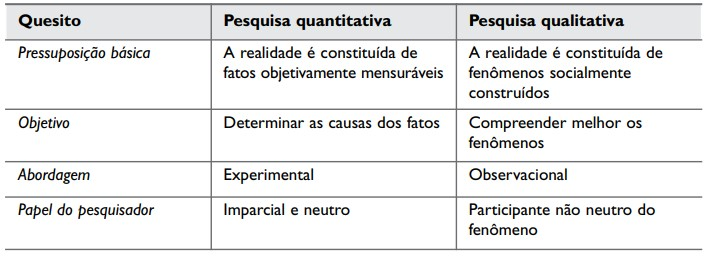
\includegraphics[scale=0.6]{Figuras/02_natureza_pesquisa.jpg}
    \label{fig:natureza_pesquisa}
\end{figure}

\end{ftst}

%=====

\begin{ftst}{Quanto aos objetivos da pesquisa}{Métodos de Pesquisa}
\vone
\justifying
A \textcolor{blue}{pesquisa exploratória} é aquela em que o autor não tem necessariamente uma hipótese ou objetivo definido em mente. 
\vone
Ela pode ser considerada, muitas vezes, como o primeiro estágio de um processo de pesquisa mais longo. 
\vone
Na pesquisa exploratória, o autor vai examinar um conjunto de fenômenos, buscando anomalias que não sejam ainda conhecidas e que possam ser, então, a base para uma pesquisa mais elaborada.
\vone


\end{ftst}

%=====

\begin{ftst}{Quanto aos objetivos da pesquisa}{Métodos de Pesquisa}
\vone
\justifying
A \textcolor{blue}{pesquisa descritiva} é mais sistemática do que a exploratória. Com ela busca-se obter dados mais consistentes sobre determinada realidade, mas não há ainda interferência do pesquisador ou a tentativa de obter teorias que expliquem os fenômenos. 
\voneTenta-se
apenas descrever os fatos como são.
\vone
A pesquisa descritiva é caracterizada pelo levantamento de dados e pela aplicação de entrevistas e questionários. 
\vone
Assim como a pesquisa exploratória, ela pode ser considerada um passo prévio para encontrar fenômenos não explicados pelas teorias vigentes.

\end{ftst}

%=====

\begin{ftst}{Quanto aos objetivos da pesquisa}{Métodos de Pesquisa}
\vone
\justifying
A \textcolor{blue}{pesquisa explicativa} é a mais complexa e completa. 
\vone
É a pesquisa científica por excelência porque, além de analisar os dados observados, busca suas causas e explicações, ou seja, os fatores determinantes desses dados.


\end{ftst}

%=====

\begin{ftst}{Quanto aos procedimentos técnicos da pesquisa}{Métodos de Pesquisa}
\vone
\justifying
A \textcolor{blue}{pesquisa bibliográfica} implica o estudo de artigos, teses, livros e outras publicações usualmente disponibilizadas por editoras e indexadas.
\vone
A pesquisa bibliográfica é um passo fundamental e prévio para qualquer trabalho científico, mas ela em si não produz qualquer conhecimento novo. Apenas supre o pesquisador de informações públicas que ele ainda não possuía.


\end{ftst}

%=====

\begin{ftst}{Quanto aos procedimentos técnicos da pesquisa}{Métodos de Pesquisa}
\vone
\justifying
A \textcolor{blue}{pesquisa documental}, por outro lado, consiste na análise de documentos ou dados que não foram ainda sistematizados e publicados. Pode-se examinar relatórios de empresas, arquivos obtidos em órgãos públicos, bancos de dados, correspondências etc.
\vone
A pesquisa documental busca encontrar informações e padrões em documentos ainda não tratados sistematicamente.

\end{ftst}

%=====


\begin{ftst}{Quanto aos procedimentos técnicos da pesquisa}{Métodos de Pesquisa}
\vone
\justifying
A \textcolor{blue}{pesquisa experimental} caracteriza-se pela manipulação de um aspecto da realidade pelo pesquisador. 
\vone
O pesquisador introduz, por exemplo, uma nova técnica em uma empresa de software e observa se a produtividade aumenta. 
\vone
A pesquisa experimental implica ter uma ou mais variáveis experimentais que podem ser controladas pelo pesquisador (o fato de usar ou não determinada técnica, por exemplo), e uma ou mais variáveis observadas, cuja medição poderá levar, possivelmente, à conclusão de que existe algum tipo de dependência com a variável experimental.
\vone
A pesquisa experimental deve utilizar rigorosas técnicas de amostragem e testes de hipóteses para que seus resultados sejam estatisticamente aceitáveis e generalizáveis.

\end{ftst}

%=====

\begin{ftst}{Ciência versus tecnologia}{Métodos de Pesquisa}
\vone
\footnotesize
\justifying
Em computação, os termos ciência e tecnologia quase sempre andam tão juntos que muitas pessoas têm dificuldade em distingui-los. 
\vone
A ciência é a busca do conhecimento e das explicações, enquanto a tecnologia é a aplicação dos conhecimentos nas atividades práticas.
\vone
Observa-se que, algumas vezes, dissertações e teses em computação, bem como artigos científicos, ainda são fortemente caracterizados como apresentações meramente tecnológicas: sistemas, protótipos, frameworks, arquiteturas, modelos, processos, todas essas construções são técnicas, e não necessariamente
ciência.
\vone
Para que um trabalho seja efetivamente de cunho científico é necessário que a informação contida nele explique um pouco mais sobre o porquê de as coisas funcionarem como funcionam. 


\end{ftst}


%=====

\begin{ftst}{Referências}{Métodos de Pesquisa}
\vone
\begin{itemize}
    \item WAZLAWICK, R. S. Metodologia de Pesquisa em Ciência da Computação. Rio de Janeiro: Campus, 2009.
    \item APPOLINÁRIO, F. Metodologia da Ciência: Filosofia e Prática da Pesquisa. 2. ed. Cengage Learning, 2012.
\end{itemize} 


\end{ftst}

%=====



\end{document}